\lab{Monte Carlo Integration}{Monte Carlo Integration}
\objective{Implement Monte Carlo integration to estimate integrals. Use Monte Carlo Integration to calculate the integral of the joint normal distribution.}

Some multivariable integrals which are critical in applications are impossible to evaluate symbolically.
For example, the integral of the joint normal distribution
\[
\int_{\Omega} \frac{1}{\sqrt{(2 \pi)^k}} e^{- \frac{\bold{x}^T\bold{x}}{2}}
\]
is ubiquitous in statistics.
However, the integrand does not have a symbolic antiderivative.
This means we must use numerical methods to evaluate this integral. The standard technique for numerically evaluating multivariable integrals is \emph{Monte Carlo Integration}. In the next lab, we will approximate this integral using a modified version of Monte Carlo Integration. In this lab, we address the basics of Monte Carlo Integration.

Monte Carlo integration is radically different from 1-dimensional techniques like Simpson's rule. Whereas Simpson's rule is purely computational, Monte Carlo integration relies on probability to calculate the integral.
Although it converges slowly, Monte Carlo integration is frequently used to evaluate multivariable integrals because the higher-dimensional analogs of methods like Simpson's rule are inefficient. 

\section*{A Motivating Example}
Suppose we want to numerically compute the area of a circle of radius 1.
From analytic methods, we know the answer is $\pi$.
Empirically, we can estimate this quantity by randomly choosing points in a $2 \times 2$ square.
The percent of points that land in the inscribed circle, times the area of the square, should approximately equal the area of the circle (see Figure \ref{fig:MCCircle}).

\begin{figure}
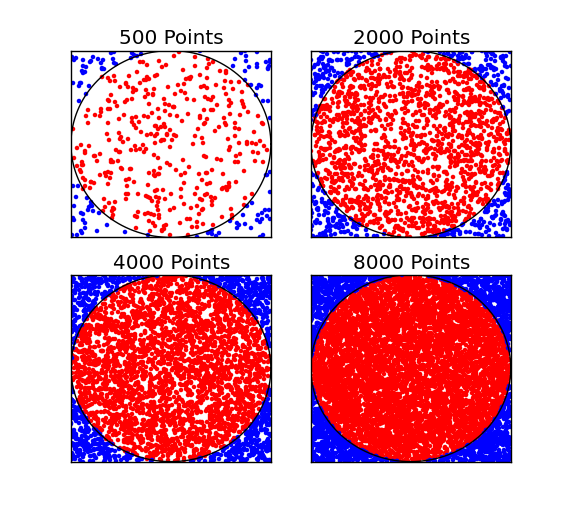
\includegraphics[width=.7\textwidth]{MC.png}
\caption{Finding the area of a circle using random points}
\label{fig:MCCircle}
\end{figure}

We do this in NumPy as follows. First generate 500 random points in the square $[0,1] \times [0,1]$.
\begin{lstlisting}
>>> numPoints = 500
>>> points = np.random.rand(2, numPoints)
\end{lstlisting}
We rescale and shift these points to be uniformly distributed in $[-1,1]\times[-1,1]$.
\begin{lstlisting}
>>> points = points*2-1
\end{lstlisting}
Next we compute the number of points in the unit circle.
The function \li{np.hypot(a, b)} returns the norm of the vector $(a, b)$ where $a$ and $b$ are the $x$- and $y$-components, respectively.
\begin{lstlisting}
>>> # Create a mask of points in the circle
>>> circleMask = np.hypot(points[0,:], points[1,:]) <= 1
>>> # Count how many there are
>>> numInCircle = np.count_nonzero(circleMask)
\end{lstlisting}
Finally, we approximate the area.
\begin{lstlisting}
>>> # Area is approximately (area of the square)*(num points in circle)/(total num points)
>>> 4.*numInCircle/numPoints
3.024
\end{lstlisting}
This differs from $\pi$ by about 0.117.

\begin{problem}
\label{prob:sphere}
Write a function that estimates the volume of the unit sphere. Your function should have a keyword argument \li{numPoints} that defaults to $10^5$. Your function should draw \li{numPoints} points uniformly from $[-1,1]\times[-1,1]\times[-1,1]$ to make your estimate. Your answer should be approximately 4.189.
\end{problem}

We analyze the error of the Monte Carlo method by repeating this experiment for many values of \li{numPoints} and plotting the errors.
The result is the blue line in Figure \ref{fig:mc_error}.
The error appears to be proportional to $1/\sqrt{N}$ where $N=$ \li{numPoints} (the green line in Figure \ref{fig:mc_error}).
This means that to divide the error by 10, we must sample \emph{100 times} more points.

\begin{figure}
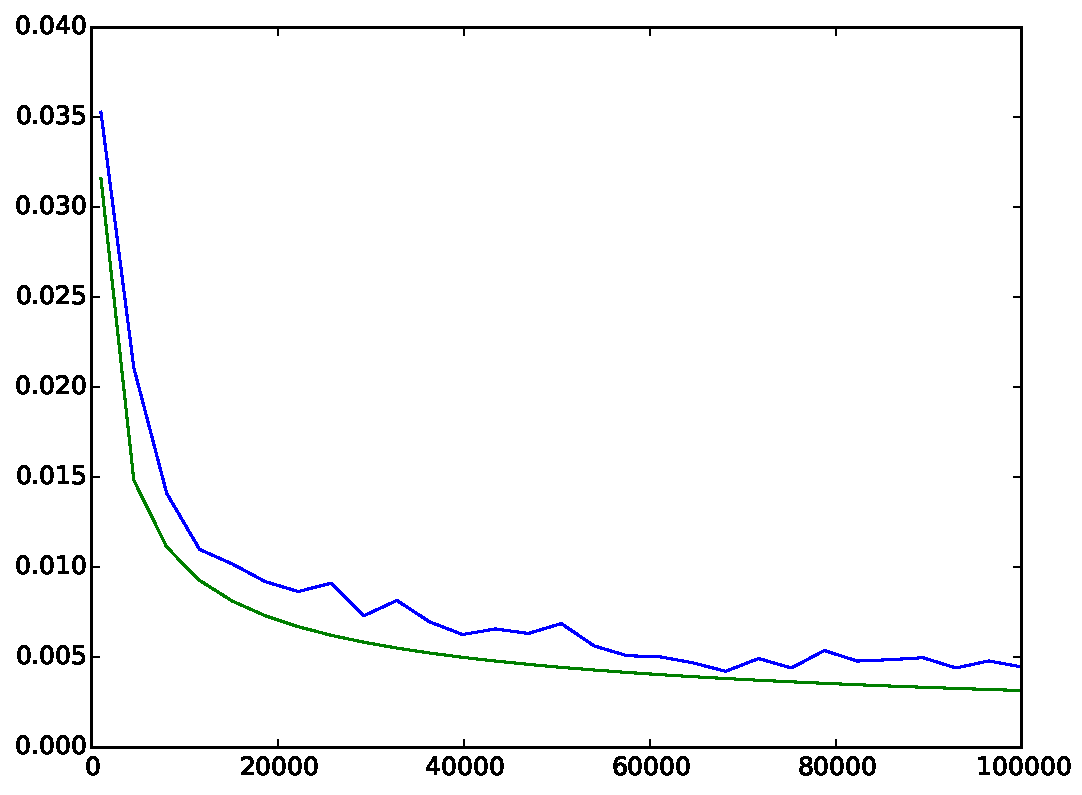
\includegraphics[width=.7\textwidth]{mc_error.pdf}
\caption{The Monte Carlo integration method was used to compute the area of a circle of radius 1. 
The blue line plots the average error in 100 runs of the Monte Carlo method on $N$ sample points, where $N$ appears on the horizontal axis.
The green line is a plot of $1/\sqrt{N}$. }
\label{fig:mc_error}
\end{figure}

This is a slow convergence rate, but it is independent of the number of dimensions of the problem. 
This dimension independence is what makes the Monte Carlo method useful for multivariable integrals.

\section*{Monte Carlo Integration}

You can calculate the area of the unit circle with the following integration problem:
\[
\mbox{Area of unit circle } = \int_{[-1,1]\times[-1,1]} f(x,y) dA
\]
where
\begin{equation}\label{equ:mc_func}
f(x,y) = \begin{cases} 1 &\mbox{ if $(x$,$y)$ is in the unit circle} \\ 0 &\mbox{ otherwise.} \end{cases}
\end{equation}
%$

This method essentially draws a box around the function to estimate the integral. This works fine if we know the bounds of the function. However, if we don't know the bounds of the function we don't know the dimensions of the box much be to encapsulate the function. 

Luckily, we can still use a random-points method as above to approximate any integral, even if we don't know the bounds. Suppose we wish to evaluate
\[
\int_\Omega f(x)\:dV.
\]
We can approximate this integral using the formula
\begin{equation}\label{equ:mc_eq}
\int_\Omega f(x)\:dV \approx V(\Omega) \frac{1}{N} \sum_{i=1}^N f(x_i),
\end{equation}
where $x_i$ are uniformly distributed random vectors in $\Omega$ and $V(\Omega)$ is the volume of $\Omega$.
This is the formula for Monte Carlo integration. 


In our example, $\Omega$ was the box $[-1,1] \times [-1,1]$ and $f$ was the function defined in \eqref{equ:mc_func}.
Then $\sum_{i=1}^N f(x_i)$ is the number of points in the unit circle, $N$ is the total number of points, and \eqref{equ:mc_eq} is the same as the formula we derived previously.

The intuition behind \eqref{equ:mc_eq} is that $\frac{1}{N} \sum_{i=1}^N f(x_i)$ approximates the average value of $f$ on $\Omega$.
We multiply this (approximate) average value by the volume of $\Omega$ to get the (approximate) integral of $f$ on $\Omega$.

As a 1-dimensional example consider the integral 
\[
\int_0^1 x\,dx \approx (1-0)\frac{1}{N} \sum_{i=1}^N x_i=\frac{1}{N} \sum_{i=1}^N x_i.
\]

The integral on the left-hand-side is $1/2$. 
In the approximation on the right-hand-side, $x_i$ is drawn from a uniform distribution on $[0,1]$. 
The average of $N$ such draws will converge to $1/2$. 

\begin{problem}
\label{prob:crazy_sine}
Monte Carlo Integration is particularly useful when trying to approximate integrals that would be difficult to calculate otherwise. Write a function that approximates the following integral:
$$\int_{1}^{5} \left | \text{sin}(10x)\text{cos}(10x) + \sqrt{x}\text{sin}(3x) \right | dx$$
Your function should accept a keyword argument \li{numPoints} that defaults to $10^5$. Your answer should be approximately $4.502$.
\end{problem}

\begin{problem}
\label{prob:mc}
Implement Monte Carlo integration with the following function. Your implementation should be robust enough to integrate any function $f$ : $\mathbb{R}^n \rightarrow \mathbb{R}$ over any interval in $\mathbb{R}^n$.
Your implementation should run the Monte Carlo algorithm several times 
and return the average of those runs. Test your function by recalculating Problem 1 and 2.
\begin{lstlisting}
def mc_int(f, mins, maxs, numPoints=500, numIters=100):
    """Use Monte Carlo integration to approximate the integral of f
    on the box defined by mins and maxs.
    
    Inputs:
        f (function) - The function to integrate. This function should 
            accept a 1-D NumPy array as input.
        mins (1-D np.ndarray) - Minimum bounds on integration.
        maxs (1-D np.ndarray) - Maximum bounds on integration.
        numPoints (int, optional) - The number of points to sample in 
            the Monte Carlo method. Defaults to 500.
        numIters (int, optional) - An integer specifying the number of 
            times to run the Monte Carlo algorithm. Defaults to 100.
        
    Returns:
        estimate (int) - The average of 'numIters' runs of the 
            Monte Carlo algorithm.
                
    Example:
        >>> f = lambda x: np.hypot(x[0], x[1]) <= 1
        >>> # Integral over the square [-1,1] x [-1,1]. Should be pi.
        >>> mc_int(f, np.array([-1,-1]), np.array([1,1]))
        3.1290400000000007
    """
\end{lstlisting}

Hints:
\begin{enumerate}
\item To create a random array of points on which to evaluate \li{f}, first create a random array of points in $[0,1] \times \ldots \times [0,1]$.
Then multiply this array by a vector of the lengths of the sides to stretch it the right amount in each direction.
Finally, add the appropriate vector to shift the points to the right location.
\item You can evaluate \li{f} on an array of points using \li{np.apply_along_axis()} as follows:
\begin{lstlisting}
# to evaluate the function f using the rows of vecs as input
>>> f = lambda x: la.norm(x)
>>> vecs = np.array([[1,1,1],[0,2,1],[0.5,0.5,0.5],[1,0,1]])
>>> np.apply_along_axis(f,1,vecs)
array([ 1.73205081,  2.23606798,  0.8660254 ,  1.41421356])
\end{lstlisting}
In this example, we chose the axis parameter to be 1 to evaluate the rows of the matrix. If you would like a refresher on axes, see Lab \ref{lab:NumPyArrays}.

\end{enumerate}
\end{problem}

\begin{problem}
\label{prob:mc_test}
The exact value of the integral of
\[
f(x,y,z,w) = \text{sin}(x) y^5 -y^3 + zw + yz^3
\]
on $[-1,1]\times[-1,1]\times[-1,1]\times[-1,1]$ is 0.
Run the function \li{mc_int()} you wrote in Problem 3 on $f$ with 100, 1000, and 10000 sample points. Use the default value of 100 iterations for your approximations.
Print the errors of your estimates to the terminal.
\end{problem}

\begin{comment}
One application of Monte Carlo integration is integrating probability density functions that do not have closed form solutions.

\begin{comment}
\begin{problem}
The standard normal distribution is an important object of study in probability and statistic.
It is defined by the density function $\frac{1}{\sqrt{2 \pi}} e^{- \frac{x^2}{2}}$.
(Here we are assuming a mean of $0$ and a variance of $1$).
This is a function that cannot be integrated symbolically.
We can use monte carlo integration to estimate the probability that a normally distributed random variable will take a value below a given point.
The probability that the random variable we are considering is less than (or equal to) a given value $x$ is
\[\int_{-\infty}^x \frac{1}{\sqrt{2 \pi}} e^{- \frac{t^2}{2}} dt\]
This function is essentially zero for values of $x$ that lie reasonably far from the mean, so we can estimate this probability by integrating from $-5$ to $x$ instead.

Compare your result at $x = 1$ with the output of the code
\begin{lstlisting}
from scipy.stats import norm
N = norm()
N.cdf(1)
\end{lstlisting}
\end{problem}


\begin{problem}
The joint normal distribution of $N$ independent random variables with mean 0 and variance 1 is
\[
f(\x) = \frac{1}{\sqrt{(2 \pi)^N}} e^{- \frac{\x^T\x}{2}}.
\]
The integral of $f(\x)$ over a box is the probability that a draw from the distribution will be in the box.
However, $f(\x)$ does not have a symbolic antiderivative.
\begin{enumerate}
\item The integral of this function on $B = [-1,1]\times [-1,1]\times[-1,1] \subset \mathbb{R}^3$ can be computed in SciPy with the following code.
\begin{lstlisting}
>>> import scipy.stats as stats

# Define the bounds of the box to integrate over
>>> mins = np.array([-1, -1, -1])
>>> maxs = np.array([1, 1, 1])

# Each variable has mean 0
>>> means = np.zeros(3)

# The covariance matrix of N independent random variables
#    is the NxN identity matrix.
>>> covs = np.eye(3)

# Compute the integral
>>> value, inform = stats.mvn.mvnun(mins, maxs, means, covs)
\end{lstlisting}
Then \li{value} is the integral of $f(\x)$ on $B$.
Use SciPy to integrate $f(\x)$ on $\Omega=[-0.5, 0.75]\times[0,1]\times[0, 0.5]\times[0,1] \subset \mathbb{R}^4$.

\item Use the function \li{mc_int()} you wrote in Problem \ref{prob:mc} to integrate $f(\x)$ on $\Omega$ with 10, 100, 1000, and 10,000 sample points. 
Compare the errors of your estimates to the result you got from the SciPy package.
\end{enumerate}
\end{problem}
\end{comment}

\section*{A Caution}
You can run into trouble if you try to use Monte Carlo integration on an integral that does not converge.
For example, we may attempt to evaluate
\[
\int_0^1 \frac{1}{x}
\]
with Monte Carlo integragtion using the following code.
\begin{lstlisting}
>>> k = 5000
>>> np.mean(1/np.random.rand(k,1))
21.237332864358656
\end{lstlisting}

Since this code returns a finite value, we could assume that this integral has a finite value.
In fact, the integral is infinite.
We could discover this empirically by using larger and larger values of $k$, and noting that Monte Carlo integration returns larger and larger values.

\begin{comment}
\begin{problem}
\label{prob:mc_flawed}
Create a new function (based upon the function from Problem \ref{prob:mc}) that uses a ``flawed'' random number generator that doesn't produce numbers between $-.95$ and $-1$. Test your method on the function from Problem \ref{prob:mc_test}. How bad is the error? 
\end{problem}
\end{comment}
